\documentclass[thesis.tex]{subfiles}

\chapter{Cơ sở lý thuyết}
Chương 2 trình bày cơ sở lý thuyết về học máy, học sâu, và phương pháp trích xuất đặc trưng âm học từ tín hiệu giọng nói. Đây là nền tảng để xây dựng mô hình trong chương 3.

\section{Học máy}

\subsection{Tổng quan về học máy}

Học máy (Machine learning - ML) là một nhánh con của trí tuệ nhân tạo. Nghiên cứu học máy tập trung phát triển và xây dựng các thuật toán và kỹ thuật để giúp chương trình máy tính có thể "học" thực thi một tác vụ nào đó từ kinh nghiệm. Trong \cite{mitchell1997machine}, nhà tiên phong về học máy Tom M. Mitchell định nghĩa như sau: Một chương trình máy tính được nói là học từ kinh nghiệm \textit{E} để thực thi một tác vụ \textit{T} nếu khả năng của chương trình được đo bằng độ đo \textit{P} tiến bộ với kinh nghiệm \textit{E}. Rõ ràng hơn, học máy là những chương trình máy tính có thể tự học được dữ liệu mà không cần được lập trình một cách cụ thể.

Với các cách định nghĩa \textit{T}, \textit{P}, và \textit{E} khác nhau, các thuật toán học máy có thể được phân vào các nhóm: học có giám sát, học không giám sát, học bán giám sát, và học tăng cường.

\textbf{Học có giám sát} là lớp các thuật toán sử dụng dữ liệu được gán nhãn từ trước để tìm mối liên hệ giữa đầu vào và đầu ra. Mục tiêu của học có giám sát là tạo ra mô hình có thể dự đoán được đầu ra cho các đầu vào mới mà mô hình chưa gặp bao giờ. Tập dữ liệu gán nhãn trên được gọi là dữ liệu huấn luyện. Cho tập dữ liệu huấn luyện gồm $N$ ví dụ $D = \{(\bm{x}_1, y_1), ..., (\bm{x}_N, y_N)\}$ trong đó $\bm{x}_i$ là vec-tơ đặc trưng của ví dụ thứ $i$ và $y_i$ là nhãn tương ứng. Thuật toán học có giám sát tìm hàm ánh xạ $f: X \longrightarrow Y$ trong đó $X$ là không gian vec-tơ đầu vào và $Y$ là tập các nhãn. 

Các thuật toán học có giám sát thường được sử dụng để giải quyết hai loại bài toán: phân loại (classification) và hồi quy (regression). Bài toán phân loại có nhãn rời rạc thuộc một tập cho sẵn. Ví dụ: phân loại đồ vật, phân loại phương tiện giao thông, phân loại giới tính dựa trên giọng nói. Khác với bài toán phân loại, bài toán hồi quy lại có nhãn nằm trên một miền liên tục. Ví dụ: dự đoán giá nhà đất, dự đoán thị trường chứng khoán.

Trong \textbf{học không giám sát}, khác với học có giám sát, ta chỉ có dữ liệu đầu vào mà không có dữ liệu đầu ra. Mục tiêu chính của các thuật toán là tìm ra cấu trúc ẩn trong dữ liệu hoặc trích xuất đặc trưng chung của tập dữ liệu.

\textbf{Học bán giám sát} nằm giữa học có giám sát và không có giám sát. Học bán giám sát thường được sử dụng khi có một lượng lớn dữ liệu không có nhãn và một số ít dữ liệu có nhãn. Phương pháp học bán giám sát được sử dụng rộng rãi nhất - tự huấn luyện (self-training) sử dụng mô hình huấn luyện trên tập có nhãn để sinh nhãn giả từ tập không nhãn nhằm tăng cường khả năng học của mô hình.

Hệ thống \textbf{học củng cố} được xem như là một tác tử trong một môi trường vô định và phức tạp. Với mỗi hành động, tác tử này nhận điểm thưởng hoặc phạt từ môi trường. Mục tiêu của học củng cố là các tác tử thông minh để tối đa điểm thưởng và thực hiện tác vụ của nó. Học củng cố hiện đang là lĩnh vực nghiên cứu tập trung nhiều nguồn lực và công sức với nhiều ứng dụng thực tế liên quan tới điều khiển robot hay vận hành nhà máy một cách tự động.

\subsection{Mạng nơ-ron nhân tạo}\label{ann}
Mạng nơ-ron nhân tạo (Artificial Neural Networks - ANN) là một mô hình tính toán mô phỏng cách nơ-ron trong não người phân tích và xử lý thông tin. Học sâu với nền tảng là ANN cho phép xử lý dữ liệu và thông tin với độ chính xác vượt xa các mô hình xác suất cổ điển và tốc độ vượt trội so với con người. 

Nơ-ron sinh học gồm 3 phần chính: dendrite, thân tế bào (soma) và axon (Hình \ref*{fig:neuron}). Đầu tiên, tín hiệu đầu vào được thu thập bởi các khớp thần kinh của dendrite. Vai trò của soma là xử lý đầu vào và tổng hợp thông tin dựa vào độ quan trọng của tín hiệu. Sau đó, axon sẽ truyền thông tin đã được xử lý tới đầu ra. Thành phần cấu thành nên ANN là perceptron cũng có cách thức hoạt động tương tự. Perceptron bao gồm lớp đầu vào, tập trọng số cùng hàm kích hoạt để tổng hợp thông tin và lớp đầu ra, tương tự như dendrite, soma và axon.

\begin{figure}[h]
  \centering
  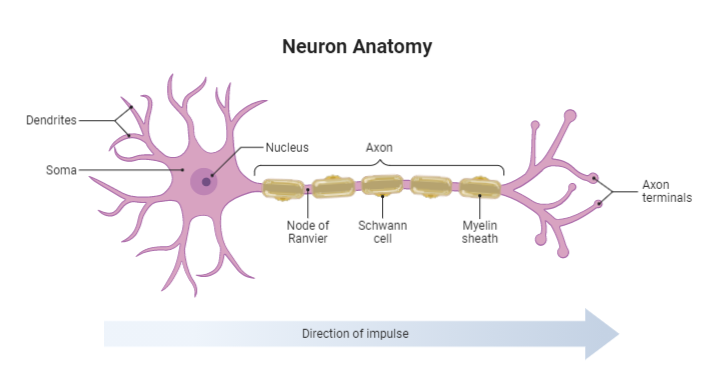
\includegraphics[width=1.0\textwidth]{images/neuron.png}
  \caption{Cấu tạo nơ-ron sinh học \protect\footnotemark.}
  \label{fig:neuron}
\end{figure}
\footnotetext{https://app.biorender.com/biorender-templates/t-5f5b7e6139954000b2bde860-neuron-anatomy}

Mạng nơ-ron là mô hình gồm nhiều lớp chồng lên nhau, mỗi lớp bao gồm nhiều perceptron (hay nơ-ron) tổng hợp thông tin từ lớp trước, mỗi lớp có một tập các nơ-ron độc lập. Lớp đầu tiên trong mạng được gọi là lớp đầu vào (input layer), lớp cuối cùng được gọi là lớp đầu ra (output layer), các lớp ở giữa được gọi là lớp ẩn (hidden layer) (Hình \ref{fig:neuron}). 

\begin{figure}[h]
  \centering
  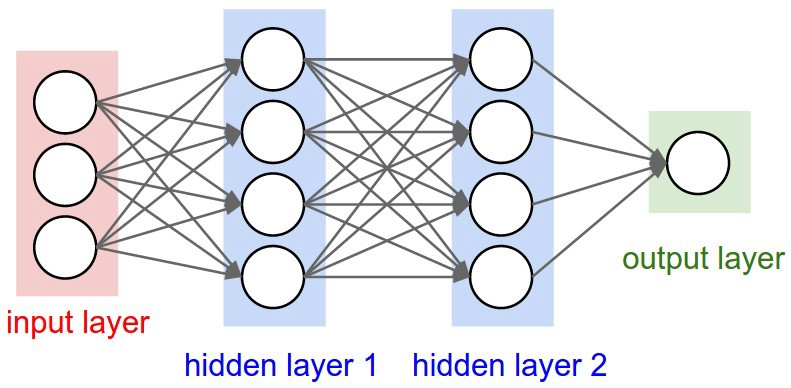
\includegraphics[width=0.6\textwidth]{images/artificial-neural-network.jpeg}
  \caption{Cấu trúc của mạng nơ-ron nhân tạo\protect\footnotemark.}
  \label{fig:neuron}
\end{figure}
\footnotetext{https://towardsdatascience.com/vanilla-neural-networks-in-r-43b028f415}

Cho một mạng nơ-ron nhân tạo gồm $L$ lớp, với $\bm{a}^i$ là tập các nơ-ron trong lớp thứ $i$, hai lớp nơ-ron liên tiếp có chỉ số $i$ và $i+1$ được kết nối với nhau bằng một ma trận trọng số $\bm{W}^i$ và một vec-tơ bias $\bm{b}^i$. Ta có thể mô tả quá trình tính toán các nơ-ron từ lớp đầu vào và đầu ra dưới dạng toán học như trong Công thức \ref{eq:fc}.

\begin{equation}\label{eq:fc}
  \bm{a}^{(i)} = \sigma(\bm{W}^i\bm{a}^{(i-1)} + \bm{b}^i),\ 0 \le i \le L 
\end{equation}

Trong đó, $\sigma$ được gọi là hàm kích hoạt (activation function). Hàm kích hoạt là một thành phần quan trọng không thể thiếu trong mạng nơ-ron nhân tạo. Để mạng nơ-ron nhân tạo có thể xấp xỉ hay học được những biến đổi phức tạp, $\sigma$ phải là một hàm phi tuyến. Nếu không có hàm kích hoạt hay hàm kích hoạt là tuyến tính thì mạng nơ-ron dù có nhiều lớp đến đâu cũng có thể quy về một hàm tuyến tính và không có khả năng học được nhiều thông tin từ dữ liệu.

Có rất nhiều hàm kích hoạt khác nhau, ví dụ như hàm ReLU, hàm sigmoid, hàm Tanh, hàm softplus,... Trong các mạng nơ-ron hiện đại, hàm ReLU \cite{nair2010rectified} (Công thức \ref{eq:relu}) được sử dụng phổ biến nhất do có nhiều lợi ích cho quá trình huấn luyện và tốc độ tính toán nhanh.

\begin{equation}\label{eq:relu}
  ReLU(x)=\max (0, x)
\end{equation}

Quá trình lần lượt tính toán mạng nơ-ron từ lớp đầu vào, tới lớp ẩn và cuối cùng là lớp đầu ra được gọi là quá trình lan truyền tiến (feedforward). 

Mạng nơ-ron học từ quá trình đối nghịch với lan truyền tiến gọi là lan truyền ngược (backpropagation). Với vec-tơ đặc trưng đầu vào $\bm{x}$ với nhãn tương ứng $y$, đầu tiên ta tính giá trị của nơ-ron lớp đầu ra $\bm{a}^{L-1}$ bằng quá trình lan truyền tiến. Sau đó, ta "lan truyền" sai khác giữa $\bm{a}^{L-1}$ và $y$ tới toàn mạng để điều chỉnh các bộ trọng số $\bm{W}^i$ và $\bm{b}^i$ với mục tiêu để giảm sai khác này.

Để đo đạc sự sai khác trong đầu ra của mạng và nhãn đầu vào, ta sử dụng một hàm mất mát. Dựa vào tác vụ khác nhau của bài toán ta cần sử dụng các hàm mất mát khác nhau. Thông thường, bài toán hồi quy sử dụng hàm trung bình bình phương sai số (Mean Square Error - MSE), còn bài toán phân loại sử dụng hàm entropy chéo (Cross Entropy - CE). Với tập dữ liệu $D = \{(\bm{x}_1, y_1), ..., (\bm{x}_N, y_N)\}$, giả sử lớp cuối cùng của mạng có một nơ-ron, gọi $a^{L-1}_i$ là giá trị của nơ-ron đầu ra tương ứng với dữ liệu đầu vào $\bm{x}_i$. Hàm mất mát MSE được tính trong Công thức \ref*{eq:mse}.

\begin{equation}\label{eq:mse}
  MSE = \dfrac{1}{N} \sum_{i=1}^N (y_i - a^{L-1}_i)^2
\end{equation}

Hàm CE được tính theo Công thức \ref*{eq:ce}.

\begin{equation}\label{eq:ce}
  CE = -\dfrac{1}{N} \sum_{i=1}^N a^{L-1}_i log(y_i)
\end{equation}

Để điều chỉnh các trọng số, ta cần phải biết giá trị cập nhật cho mỗi trọng số. Dựa trên giá trị mất mát, các tín hiệu mất mát của nơ-ron trong lớp thứ $i$ được tính toán dựa trên lỗi mà lớp thứ $i+1$ gây ra. Tín hiệu mất mát này được lan truyền từ lớp đầu ra về tới lớp đầu vào, sau đó thực hiện cập nhật các trọng số $\bm{W}, \bm{b}$ nhằm giảm các giá trị lỗi. Các giá trị lỗi của các bộ trọng số được gọi là gradient. 

Sau khi có bộ gradient, ta có thể cập nhật mạng bằng cách đi ngược lại với hướng của gradient. Giá trị mất mát trên bộ dữ liệu sẽ giảm nếu gradient được cập nhật với bước đủ nhỏ. Bằng cách lặp đi lặp lại quá trình lan truyền tiến, lan truyền ngược và cập nhật trọng số bằng gradient, bộ trọng số có thể hội tụ tại một điểm cực tiểu của hàm mất mát. Phương pháp tối ưu lặp này được gọi là gradient descent (Hình \ref*{fig:gradient-descent}).

\begin{figure}[h]
  \centering
  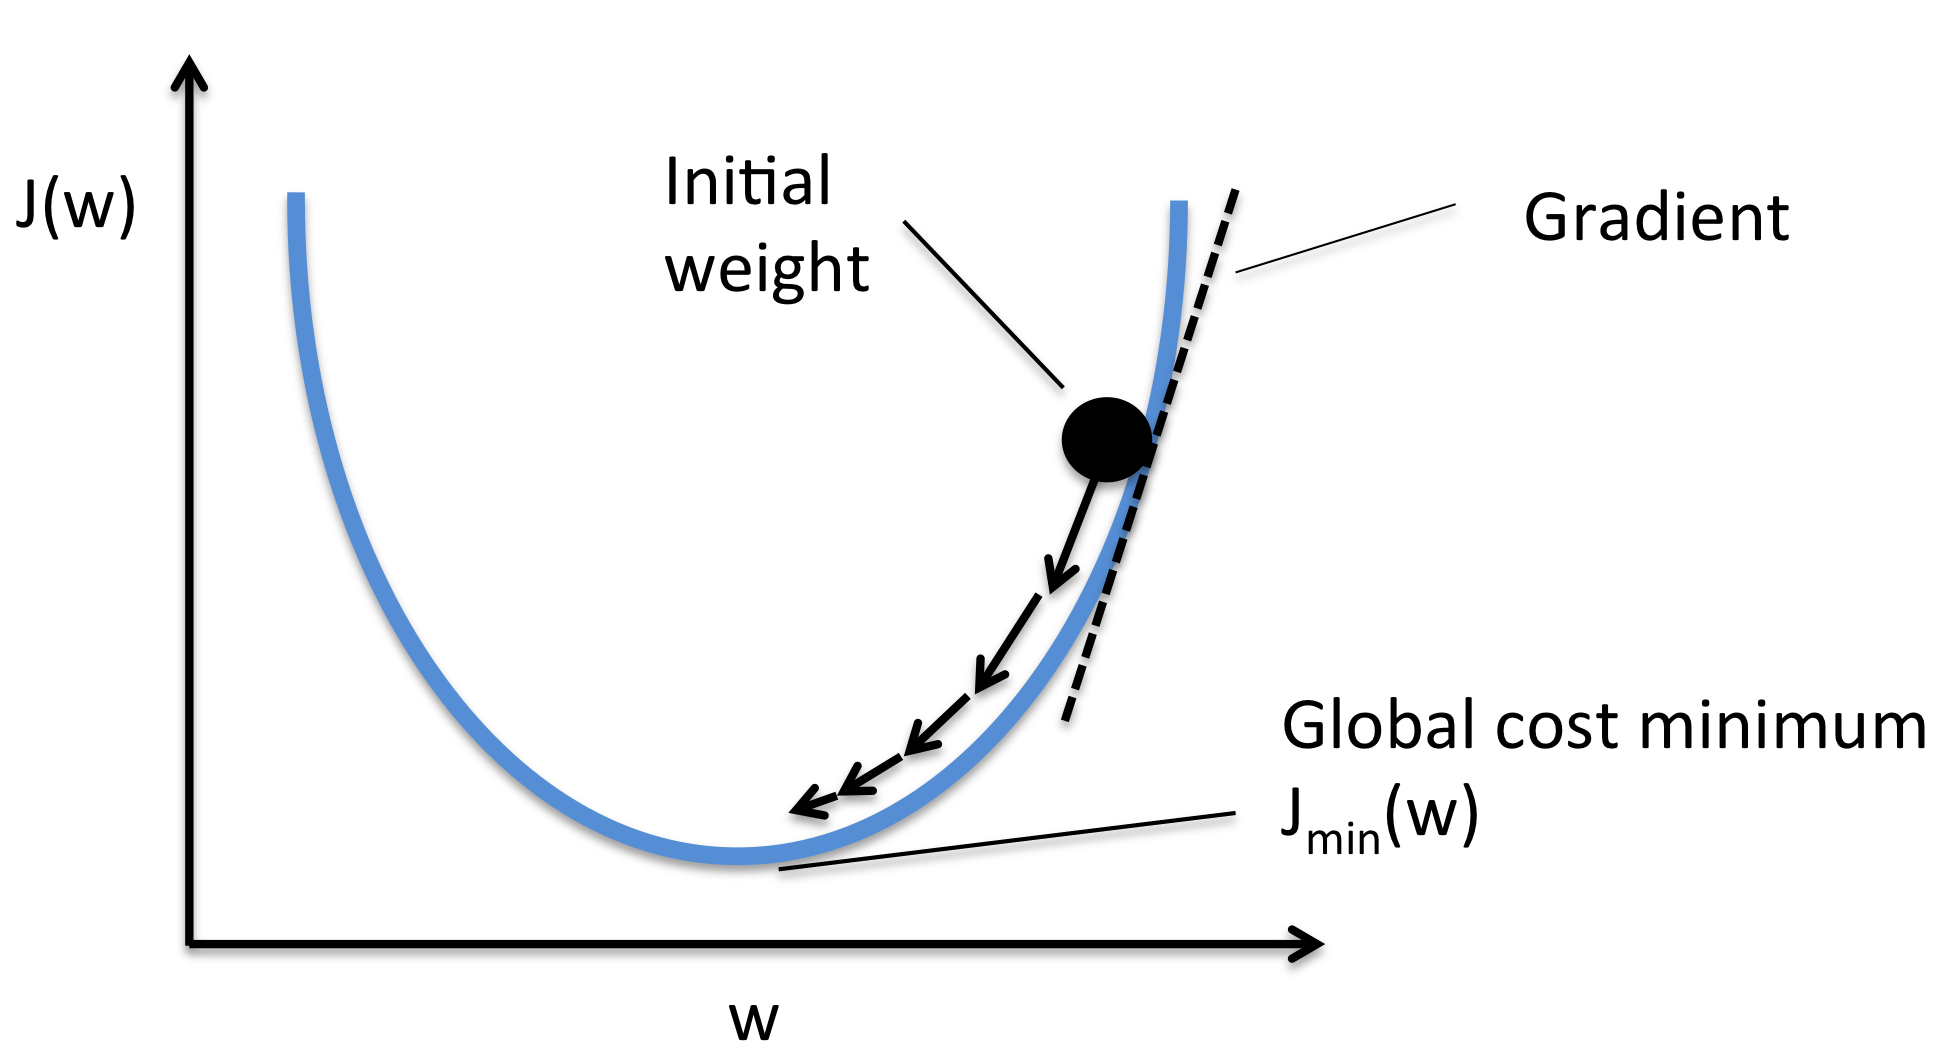
\includegraphics[width=0.6\textwidth]{images/gradient-descent.png}
  \caption{Phương pháp gradient descent \protect\footnotemark.}
  \label{fig:gradient-descent}
\end{figure}
\footnotetext{https://machinelearningnotepad.wordpress.com/2018/04/15/gradient-descent}

Hệ số học (learning rate) được điều chỉnh để kiểm soát bước cập nhật trong gradient descent. Với hệ số học lớn, bước đi của gradient descent trở nên lớn hơn và có thể gặp khó khăn hội tụ khi gần điểm cực tiểu. Hệ số học nhỏ hơn giúp mô hình dễ hội tụ hơn tuy nhiên mất nhiều vòng lặp hơn. 

Phương pháp gradient descent truyền thống sử dụng gradient cho cả bộ dữ liệu. Tuy vậy, với các bộ dữ liệu cực lớn, điều này là không thể. Do vậy, ta phải xấp xỉ gradient của cả bộ dữ liệu bằng cách chia nhỏ bộ dữ liệu gốc thành các lô nhỏ (mini-batch) và thực hiện việc cập nhật trọng số trên các lô này. Phương pháp xấp xỉ này được gọi là stochastic gradient descent - SGD. Gần đây, nhiều phương pháp biến thể của SGD được phát triển có thể kể đến như RMSprop, Adadelta \cite{zeiler2012adadelta} và Adam \cite{kingma2014adam} giúp tăng tốc độ hội tụ cũng như tăng cường hiệu năng khi huấn luyện mô hình.

\section{Học sâu}\label{deep-learning}

Học sâu là một lớp các mô hình học máy được xây dựng dựa trên mạng nơ-ron nhân tạo. Nếu mạng nơ-ron nhân tạo chỉ gồm vài lớp nơ-ron, các mạng học sâu được thiết kế để mở rộng ra hàng chục, trăm, thậm chí hàng nghìn lớp nơ-ron. Điều này giúp các mô hình học sâu giải quyết được nhiều bài toán phức tạp với độ chính xác ngang bằng con người. Huấn luyện mô hình học sâu yêu cầu một lượng dữ liệu và tài nguyên tính toán cực lớn. Trong thập kỉ vừa qua với sự bùng nổ của dữ liệu và tài nguyên tính toán, nghiên cứu học sâu trở thành tâm điểm của lĩnh vực trí tuệ nhân tạo.

\subsection{Mạng nơ-ron tích chập}

Mạng nơ-ron tích chập (Convolutional Neural Networks - CNN), hay mạng tích chập, được đề xuất lần đầu vào năm 1989 bởi Yann LeCun \cite{lecun1989backpropagation} để giải quyết bài toán nhận dạng chữ viết tay. Mạng tích chập được thiết kế với mục tiêu xử lý dữ liệu dạng bảng - lưới, ví dụ như dữ liệu chuỗi thời gian có thể biểu diễn dưới dạng bảng 1D hay ảnh là dữ liệu 2D của các điểm ảnh. Năm 2012, Alex Krizhevsky xây dựng một mạng tích chập (AlexNet \cite{krizhevsky2012imagenet}) và tăng tốc quá trình huấn luyện sử dụng GPU. Mô hình đề xuất của Krizhevsky đứng đầu trong bảng xếp hạng trong cuộc thi phân loại ảnh ImageNet \cite{deng2009imagenet} với độ chính xác vượt hơn 10\% các đội tham gia. Hiện nay, mạng tích chập được áp dụng xử lý nhiều bài toán phức tạp trong xử lý ảnh, xử lý ngôn ngữ tự nhiên, xử lý tín hiệu âm thanh, ...

\begin{figure}[h]
  \centering
  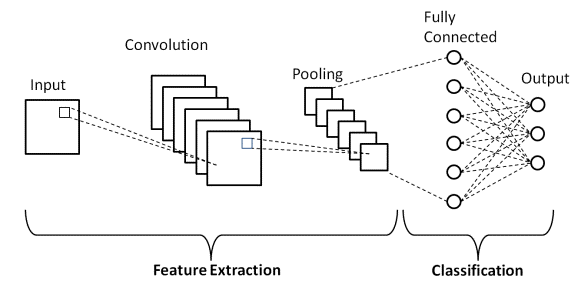
\includegraphics[width=0.8\textwidth]{images/convnet.png}
  \caption{Các thành phần cơ bản của mạng tích chập \protect\footnotemark.}
  \label{fig:convnet}
\end{figure}
\footnotetext{https://www.upgrad.com/blog/basic-cnn-architecture}

Thời điểm hiện tại đã có rất nhiều kiến trúc mạng nơ-ron tích chập khác nhau được xây dựng, tuy nhiên chúng đều được cấu thành từ các lớp thành phần (Hình \ref{fig:convnet}), bao gồm: lớp tích chập (convolutional layer), lớp tổng hợp (pooling layer) và lớp kết nối đầy đủ (fully connected layer).

\subsubsection{Lớp tích chập}
Lớp tích chập là lớp được sử dụng nhiều nhất trong mạng nơ-ron tích chập, mục tiêu của lớp tích chập là học các đặc trưng cục bộ từ dữ liệu đầu vào (Hình \ref{fig:convolutional-feature}). Cái tên lớp tích chập xuất phát từ việc lớp sử dụng phép biến đổi toán học tuyến tính gọi là tích chập (convolution).

\begin{figure}[h]
  \centering
  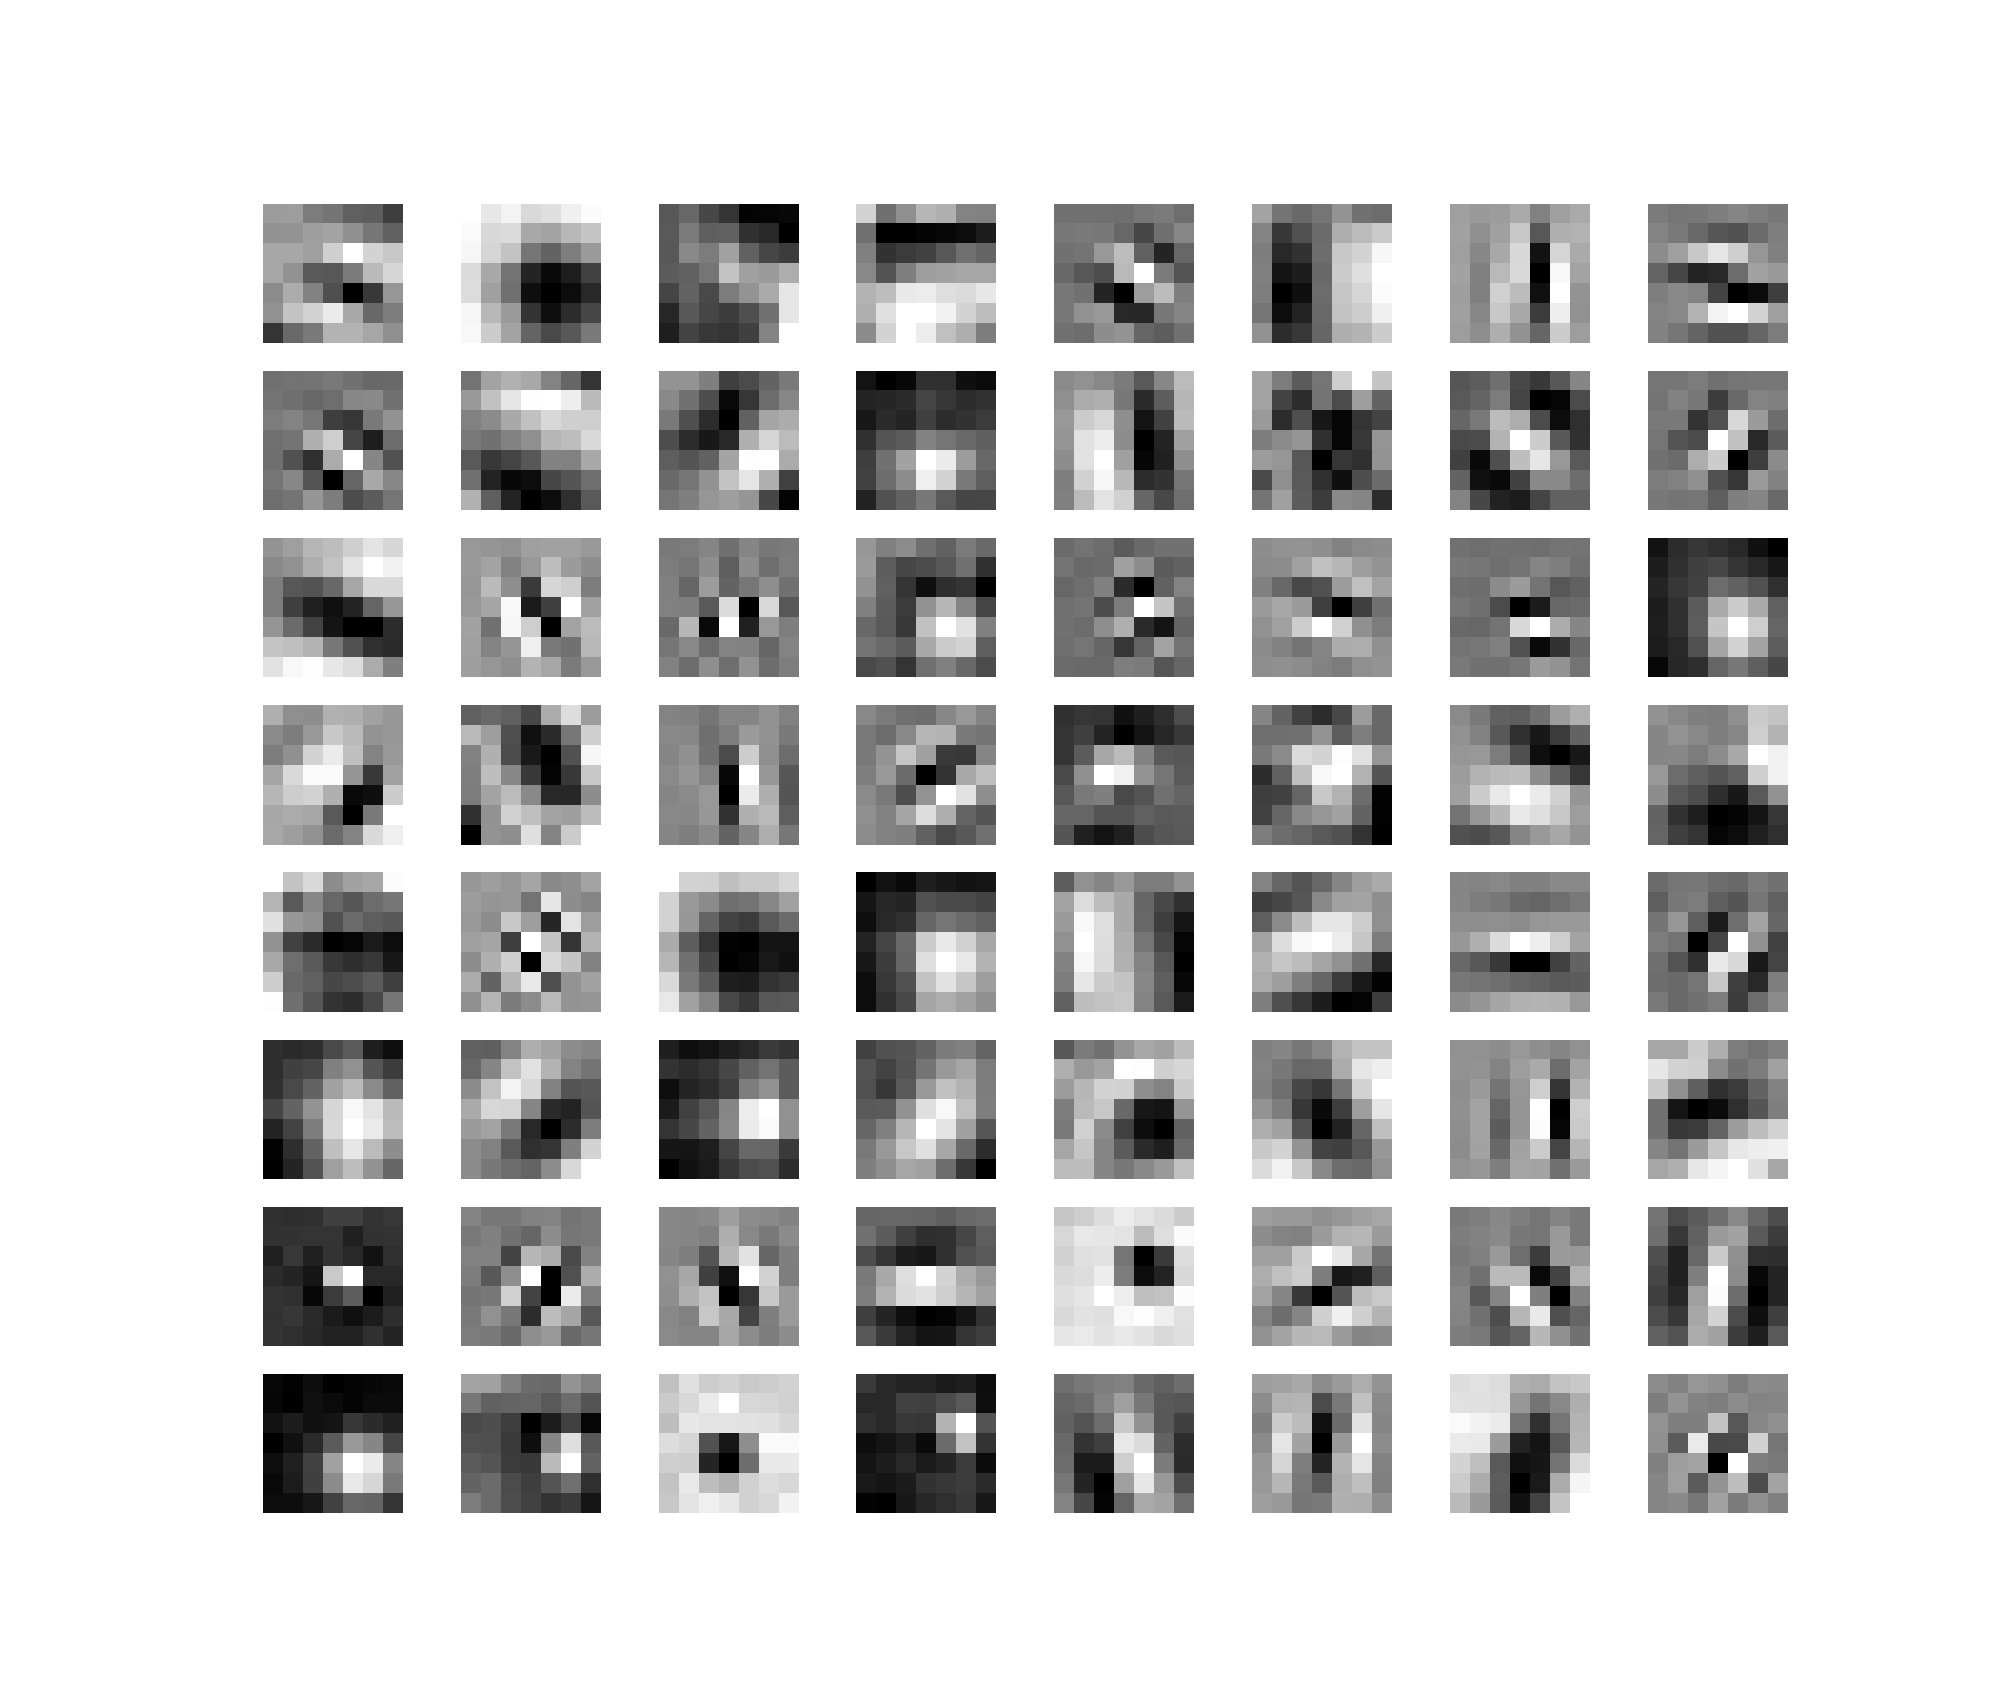
\includegraphics[width=0.7\textwidth]{images/convolutional-feature.png}
  \caption{Các đặc trưng học được trong lớp tích chập \protect\footnotemark.}
  \label{fig:convolutional-feature}
\end{figure}
\footnotetext{https://debuggercafe.com/visualizing-filters-and-feature-maps-in-convolutional-neural-networks-using-pytorch}

Ban đầu, phép tích chập được được sử dụng phổ biến trong xử lý tín hiệu. Về sau nguyên lý biến đổi trong tích chập mới được áp dụng trong lĩnh vực xử lý hình ảnh. Công thức tích chập cho 2 hàm $x$ và $w$ theo chiều thời gian $t$ được tính trong Công thức \ref{eq:convolution}.

\begin{equation}\label{eq:convolution}
  (x * w)(t)=\sum x(\alpha) w(t-\alpha)
\end{equation}

trong đó $(x * w)$ là ký hiệu tích chập. Trong xử lý ảnh, phép tích chập được mở rộng ra 2D hoặc 3D. Trong lớp tích chập, $x$ được gọi là đầu vào của lớp còn $w$ được gọi là bộ lọc (filter) (Hình \ref{fig:convolution}). Phép toán tích chập dựa trên nơ-ron của lớp trước để tính toán ra giá trị nơ-ron của lớp ngay sau.

\begin{figure}[h]
  \centering
  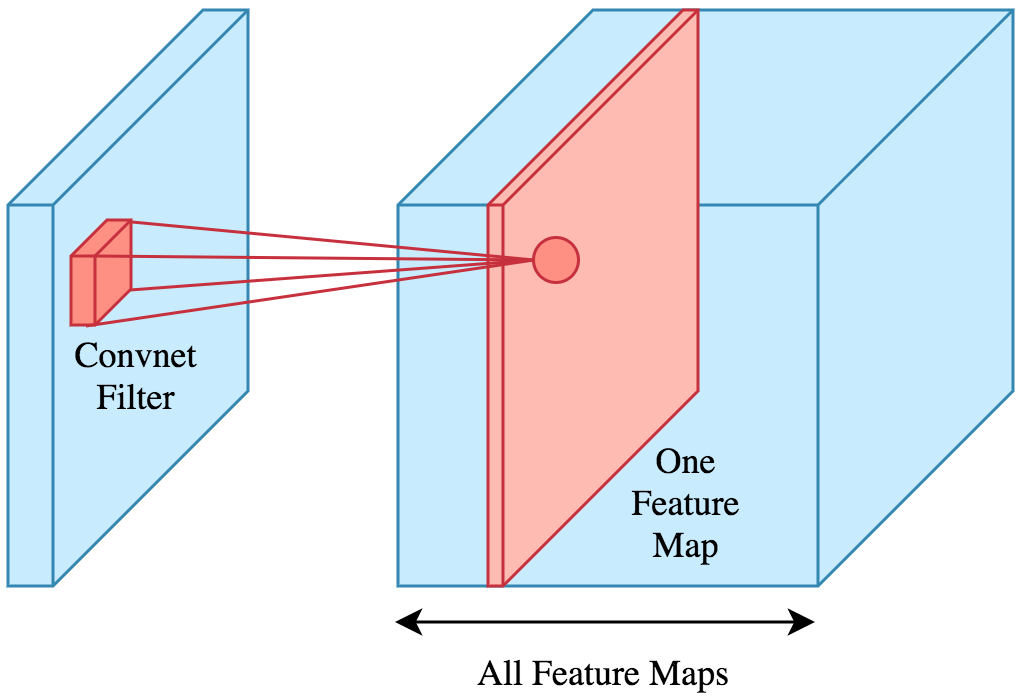
\includegraphics[width=0.6\textwidth]{images/convolution.png}
  \caption{Một ví dụ của lớp tích chập \protect\footnotemark.}
  \label{fig:convolution}
\end{figure}
\footnotetext{https://towardsdatascience.com/convolution-neural-networks-a-beginners-guide-implementing-a-mnist-hand-written-digit-8aa60330d022}

Bộ lọc là một bộ trọng số học được có kích thước nhỏ (ví dụ 5x5x3, dài rộng 5, chiều sâu 3 của khối đầu vào phía trước). Trong quá trình lan truyền tiến, bộ lọc được dịch chuyển trên cả chiều dài và chiều rộng của khối đầu vào để tổng hợp thông tin thành một khối đặc trưng 2D. Cùng với kích thước bộ lọc, lớp tích chập còn có 2 tham số bước nhảy (stride) và đệm (padding). Tham số bước nhảy quy định độ dịch chuyển của bộ lọc, còn tham số đệm là số lượng giá trị 0 được thêm vào xung quanh khối đầu vào để kiểm soát kích thước đầu ra của lớp tích chập.

Có nhiều bộ lọc trong một lớp tích chập để học nhiều dạng thông tin đặc trưng khác nhau như cạnh thẳng, cạnh chéo, đốm màu hay các đặc trưng phức tạp hơn ở các lớp sâu hơn. Các khối đặc trưng 2D của nhiều bộ lọc được xếp chồng lên nhau thành một khối đặc trưng 3D (Hình \ref{fig:convolution}).

Điểm khác biệt chính giữa lớp tích chập và lớp ẩn thông thường là tính cục bộ. Mỗi nơ-ron trong lớp tích chập chỉ được kết nối tới một số điểm nhất định trong lớp phía trước trong khi một nơ-ron trong lớp ẩn thông thường được kết nối tới tất cả nơ-ron ở lớp trước. 

Mạng tích chập giả định đặc trưng học được ở một vùng ảnh cũng có thể phát hiện đặc trưng tương tự tại một vùng khác trong ảnh. Trong quá trình tính toán tích chập, bộ trọng số của bộ lọc được sử dụng đi sử dụng lại tại các vùng khác nhau của ảnh. Điều này giúp cho tổng số trọng số của lớp tích chập ít hơn nhiều so với một lớp ẩn trong mạng nơ-ron thông thường mà vẫn học được nhiều đặc trưng ý nghĩa. Trong quá trình lan truyền ngược, gradient của bộ lọc được tổng hợp từ nhiều vùng khác nhau.

\subsubsection{Lớp tổng hợp}
Lớp tổng hợp (pooling layer) có chức năng tổng hợp thông tin từ lớp trước, giảm số nơ-ron và trọng số trong mạng từ đó giảm chi phí tính toán. Ngoài ra lớp tổng hợp còn giúp biểu diễn qua các lớp nhất quán hơn với sự thay đổi nhỏ trong đầu vào từ đó giúp mô hình hiệu quả hơn với dữ liệu mới. Cách thức hoạt động của lớp tổng hợp tương đối đơn giản, nó dùng một cửa sổ (thường có kích thước 2x2) để trượt trên đầu vào. Với mỗi điểm trượt, lớp tổng hợp chọn giá trị lớn nhất trong vùng (tổng hợp cực đại - max pooling) hoặc lấy trung bình của các giá trị (tổng hợp trung bình - average pooling) làm giá trị cho ma trận đầu ra (Hình \ref{fig:pooling}).

\begin{figure}[h]
  \centering
  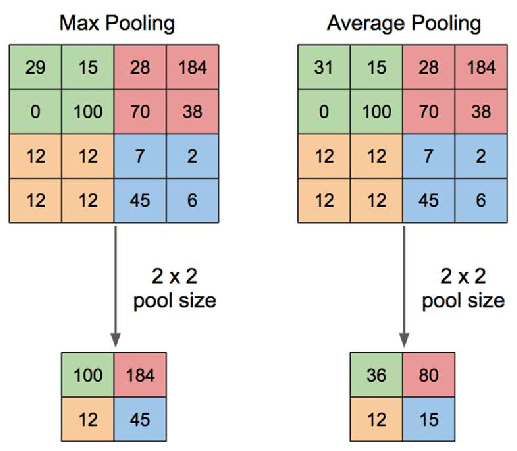
\includegraphics[width=0.6\textwidth]{images/pooling.png}
  \caption{Một ví dụ của tổng hợp cực đại và tổng hợp trung bình \cite{yani2019application}.}
  \label{fig:pooling}
\end{figure}

\subsubsection{Lớp kết nối đầy đủ}
Trong mạng nơ-ron nhân tạo thông thường, mọi lớp trừ lớp đầu vào là lớp kết nối đầy đủ, nghĩa là nơ-ron ở lớp sau được tính toán dựa trên tất cả nơ-ron của lớp trước. Thông thường trong mạng nơ-ron tích chập, lớp kết nối đầy đủ nằm ở cuối mạng, đóng vai trò là bộ phân loại của mạng. Đầu ra của lớp tích chập hay lớp tổng hợp thường là ma trận 2D hoặc 3D, do vậy cần phải được duỗi thẳng thành một vec-tơ để làm đầu vào cho lớp kết nối đầy đủ.

\subsection{Hàm mất mát}
Như đã trình bày trong phần \ref*{ann}, trong học máy, hàm mất mát đo đạc sự sai khác của đầu ra trong nhãn đầu vào. Điều tương tự cũng áp dụng cho học sâu. Trong học sâu, hàm mất mát có thể chia thành hai nhóm: hàm mất mát phân loại (classification loss) và hàm mất mát phân biệt (discriminative loss hay metric loss). Hai hàm mất mát đơn giản và được sử dụng rộng rãi nhất cho 2 nhóm là hàm softmax và hàm triplet.

\subsubsection{Hàm mất mát softmax}
Về cơ bản, hàm mất mát softmax là một hàm mất mát phân loại đa lớp gồm hàm kích hoạt softmax kết hợp hàm entropy chéo như mô tả trong Công thức \ref*{eq:ce}. Thông thường trong một mạng học sâu phân loại, lớp đầu ra có số nơ-ron tương ứng với số lớp cần được phân loại (ví dụ mô hình phân loại 6 loại xe có 6 nơ-ron ở lớp đầu ra). Giá trị đại diện cho mỗi lớp ở tầng đầu ra là cái nhận được khi sử dụng mạng dự đoán cho một ví dụ. Hàm softmax đưa vec-tơ đầu ra về khoảng $(0, 1)$ và tổng của chúng đúng bằng 1. Bởi vì giá trị của một nơ-ron đại diện cho một lớp, có thể xem đó là xác suất dự đoán của lớp đó. Hàm mất mát softmax cho một ví dụ có vec-tơ biểu diễn $\bm{z}$ thuộc lớp $c$ được tính bằng Công thức \ref{eq:softmax}.

\begin{equation}\label{eq:softmax}
  \mathcal{L}_{\text {softmax}}(\bm{z}, c) = - log(\dfrac{e^{\bm{z}_c}}{\sum_j e^{\bm{z}_j}})
\end{equation}

\subsubsection{Hàm mất mát triplet}
Khác với hàm mất mát phân loại, mục tiêu của hàm mất mát phân biệt là học điểm khác biệt giữa những vật thể hay ví dụ khác nhau. Các hàm phân biệt như triplet giúp mạng học không gian biểu diễn mà trong đó các ví dụ giống nhau sẽ gần nhau và những ví dụ khác nhau nằm xa nhau.

Đầu vào của hàm triplet bao gồm 3 điểm trong không gian biểu diễn. Trong mỗi ba điểm, có một điểm được gọi là neo (anchor) kí hiệu A, một điểm dương (positive) kí hiệu P có cùng nhãn với A, và một điểm âm (negative) kí hiệu N khác nhãn với A. Mục tiêu của hàm triplet là kéo điểm P gần hơn tới A trong không gian biểu diễn và đẩy P ra khỏi A sao cho khoảng cách A - P nhỏ hơn khoảng cách A - N một khoảng $m$ gọi là biên (margin) (Hình \ref{fig:triplet}). Với $m$ là hệ số biên, $\bm{z}_i, \bm{z}_j, \bm{z}_k$ lần vượt là vec-tơ A, P, N, giá trị hàm triplet được tính như trong Công thức \ref{eq:triplet}.

\begin{equation} \label{eq:triplet}
  \mathcal{L}_{\text {triplet }}\left(\bm{z}_{i}, \bm{z}_{j}, \bm{z}_{k}\right)=\max \left(0,\left\|\bm{z}_{i}-\bm{z}_{j}\right\|_{2}^{2}-\left\|\bm{z}_{i}-\bm{z}_{k}\right\|_{2}^{2}+m\right)
\end{equation}

\begin{figure}[h]
  \centering
  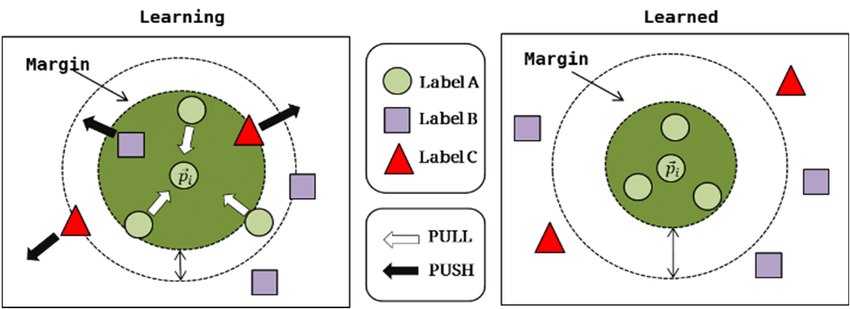
\includegraphics[width=0.8\textwidth]{images/triplet-loss.png}
  \caption{Ví dụ hàm mất mát triplet \cite{ni2017fine}.}
  \label{fig:triplet}
\end{figure}

\subsection{Mạng nơ-ron kết nối tắt}
Các mạng học sâu khi mở rộng càng nhiều lớp càng có khả năng xấp xỉ các hàm phức tạp và giải quyết bài toán phức tạp hơn. Tuy nhiên, mạng rất sâu lại gặp phải vấn đề vanishing/exploding gradients, hiện tượng mà gradient tiến tới 0 hoặc vô hạn trong quá trình lan truyền ngược trong các lớp đầu khiến cho mô hình không được cải thiện.

\begin{figure}[h]
  \centering
  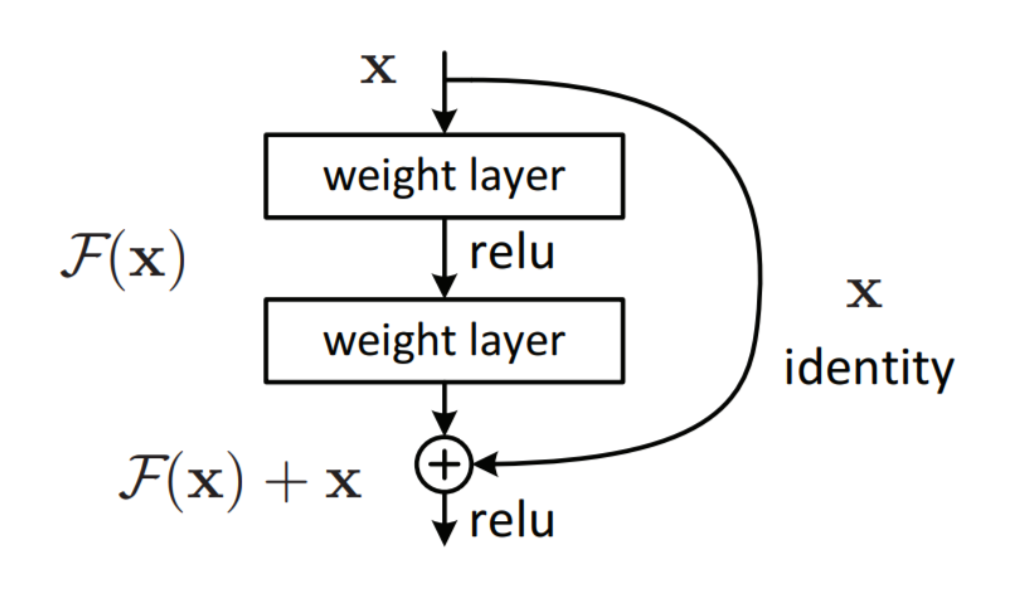
\includegraphics[width=0.6\textwidth]{images/skip-connection.png}
  \caption{Skip connection trong ResNet \cite{variani2014deep}.}
  \label{fig:skip-connection}
\end{figure}

Mạng nơ-ron kết nối tắt (Residual Neural Network - ResNet) \cite{variani2014deep} được ra đời để giải quyết vấn đề vanishing/exploding gradients. Để luồng thông tin tới được các lớp đầu của mạng trong quá trình lan truyền ngược, ResNet sử dụng một cấu trúc đặc biệt gọi là kết nối tắt (skip connection) (Hình \ref{fig:skip-connection}). Kết nối tắt khác với kết nối thông thường ở chỗ nó không kết nối 2 lớp liên tiếp mà kết nối 2 lớp không liền kề nhau. Khi lan truyền ngược, các kết nối này đưa gradient trực tiếp về các lớp phía đầu của mạng và tránh khỏi hiện tượng vanishing/exploding gradients.

\begin{figure}[h]
  \centering
  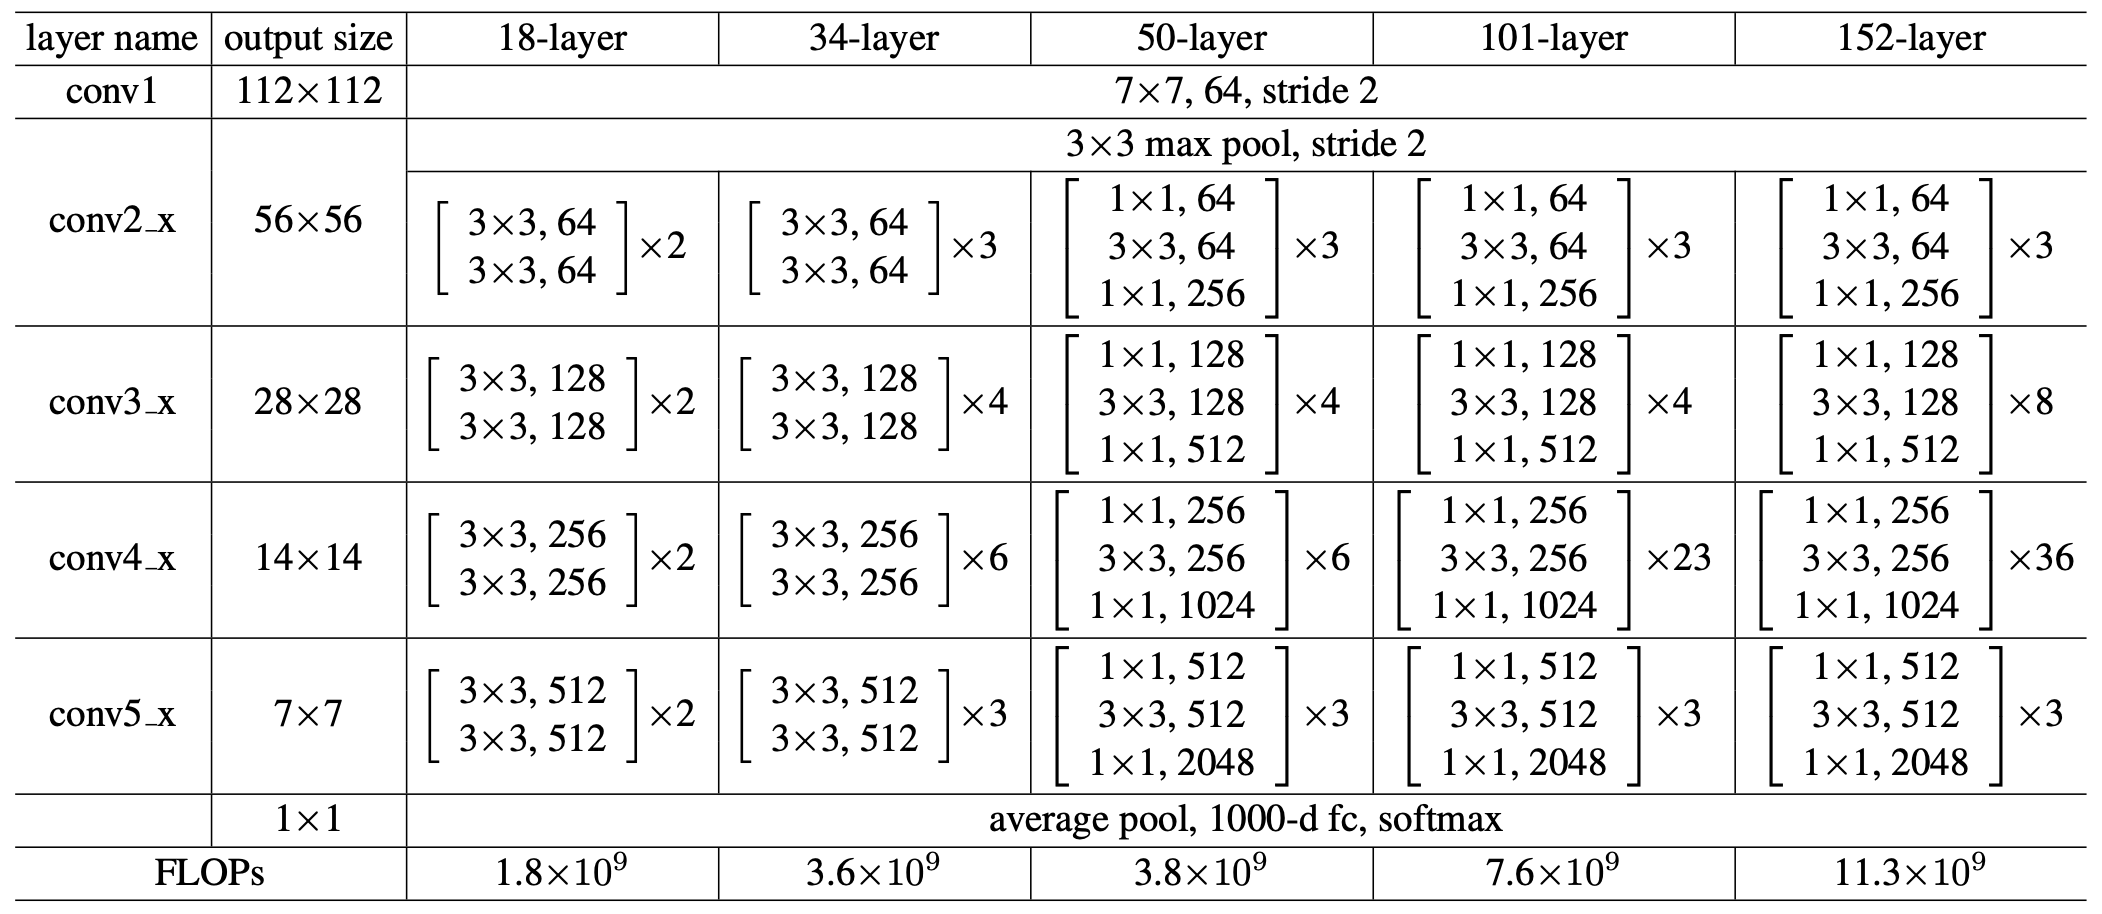
\includegraphics[width=1.0\textwidth]{images/resnet-architectures.png}
  \caption{Các kiến trúc khác nhau của ResNet \cite{variani2014deep}.}
  \label{fig:resnet-architecture}
\end{figure}

ResNet có nhiều kiến trúc với nhiều độ sâu khác nhau, hình \ref{fig:resnet-architecture} mô tả các kiến trúc này. Với ResNet-18 và ResNet-34, các khối residual được xây dựng từ các lớp tích chập với bộ lọc kích thước 3x3. Các mô hình nhiều lớp hơn như ResNet-50, ResNet-101, ResNet-152 sử dụng khối nút thắt cổ chai (bottleneck) để giảm chi chí tính toán. Hình \ref{fig:resnet-blocks} mô tả kiến trúc hai khối này.

\begin{figure}[h]
  \centering
  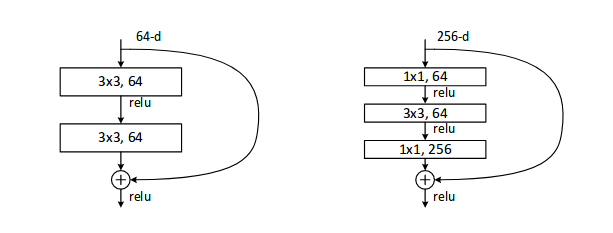
\includegraphics[width=1.0\textwidth]{images/resnet-blocks.png}
  \caption{Kiến trúc hai khối residual trong các kiến trúc mạng ResNet \cite{variani2014deep}.}
  \label{fig:resnet-blocks}
\end{figure}

\section{Trích xuất đặc trưng âm học}
Việc trích xuất đặt trưng được thực hiện bằng cách thay đổi tín hiệu giọng nói thành dạng biểu diễn tham số với tốc độ dữ liệu (data rate) tương đối thấp để dễ dàng xử lý và phân tích ở các bước sau. Trích xuất đặc trưng biến đổi tín hiệu ban đầu thành dạng ngắn gọn nhưng logic, có tính phân biệt cao và đáng tin cậy hơn tín hiệu thực. Do trích xuất đặc trưng là thành phần đầu tiên trong hệ thống, chất lượng các phần tiếp theo bị ảnh hưởng đáng kể bởi trích xuất đặc trưng.

Trích xuất đặc trưng đóng vai trò quan trọng trong bất kì hệ thống tiếng nói nào, từ nhận dạng tiếng nói tới xác minh người nói. Hai trong những đặc trưng âm thanh phổ biến nhất được sử dụng là filter banks và Mel-Frequency Cepstral Coefficients (MFCCs). 

MFCCs ban đầu được đề xuất để xác định các từ đơn âm trong các câu nói liên tục nhưng không dùng để nhận dạng người nói, xác minh người nói. Cách tính MFCCs mô phỏng hệ thống thính giác của con người nhằm tái lập nguyên lý hoạt động của tai với giả định rằng tai người là thiết bị nhận dạng người nói đáng tin cậy. MFCCs giống tai người với các bộ lọc tần số tuyến tính ở tần số thấp và logarit ở tần số cao đã được sử dụng để giữ lại các đặc tính quan trọng về mặt ngữ âm của tín hiệu giọng nói.

\begin{figure}[h]
  \centering
  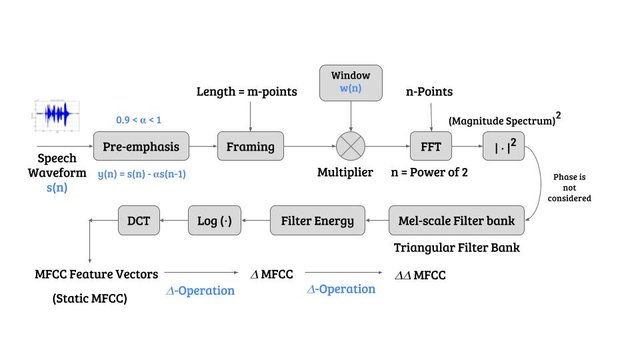
\includegraphics[width=1.0\textwidth]{images/mfcc-computation.jpg}
  \caption{Thuật toán trich xuất MFCCs \cite{barai2017asr}.}
  \label{fig:mfcc-computation}
\end{figure}

Trích xuất filter banks và MFCCs tuân theo quy trình khá tương tự nhau, trong đó cả hai trường hợp filter banks đều được tính toán và với một vài bước bổ sung có thể thu được MFCCs. Một cách ngắn gọn, một tín hiệu đi qua một bộ lọc nhấn mạnh (pre-emphasis) đầu tiên; sau đó được cắt thành các khung (frame) (chồng lên nhau) và được biến đổi bằng một loại cửa sổ (Hanning, Hamming, ...); sau đó, mỗi khung được biến đổi bằng phép biến đổi Fourier (Fourier transform) để tính toán âm phổ (spectrum) và filter banks. Để có được MFCCs, phép biến đổi cô-sin rời rạc (Disrete Cosine Transform) được áp dụng lên filter banks giữ lại một vài hệ số trong khi phần còn lại bị loại bỏ. Bước cuối cùng trong cả 2 trường hợp là chuẩn hoá trung bình (Hình \ref{fig:mfcc-computation}).

MFCCs tương đối chính xác cho các bài toán nhận diện mẫu liên quan tới giọng nói. Tuy nhiên, hiệu năng và tính khái quát hoá của MFCCs suy giảm trong trường hợp âm thanh trong thế giới thực chứa nhiều tạp âm. Ngoài ra, MFCCs còn bỏ đi thông tin cao độ của giọng nói - thông tin quan trọng để phân biệt giọng nói. Vậy nên, MFCCs không được ưa chuộng bằng filter banks trong các hệ thống nhận dạng tiếng nói hay xác minh người nói hiện đại.